\scanpage{3}
\mspage{2}
est fermé rare en $X_i$, par a) b) c)) \deleted{\unsure{est}} $\operatorname{int}(X_i)=X_i\setminus\partial X_i$, lequel est donc un ouvert \inserted{rel.} dense de $X_i$, et non vide puisque $X_i$ l'est) est \deleted{\unsure{une}} 1\textsuperscript{o}) \uuline{variété} 2\textsuperscript{o}) \uline{connexe}. (NB dans le cas $E$ modéré, on prend ``variété'' au sens modéré, certes.)
% slanted
\margin{e) Si $\deleted{X_i<X_j}\inserted{i<j}$ alors $\dim\unsure{\text{l'int}|\operatorname{int}|\operatorname{ind}}(X_i)<\dim\unsure{\operatorname{int}|\operatorname{ind}}(X_j)$, pour éviter des phénomènes de sauvagerie}
% slanted; orient the marginal drawing as on the sheet
\figure{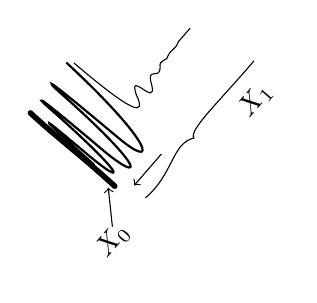
\begin{tikzpicture}[x=.85cm,y=.85cm]
\begin{scope}[rotate=49]
\draw[line width=2pt,line cap=round] (0,0) .. controls (.02,.7) and (-.02,1.15) .. (0,1.67);
\draw[line width=.8pt] (.04,.44) .. controls (.055,1.57) and (.075,1.67) .. (.09,.68)
 .. controls (.10,-.20) and (.23,-.04) .. (.24,1.60)
 .. controls (.26,1.87) and (.28,1.30) .. (.29,.49)
 .. controls (.31,-.34) and (.51,-.17) .. (.52,1.64)
 .. controls (.54,1.88) and (.56,1.58) .. (.58,.46)
 .. controls (.59,-.35) and (.86,-.05) .. (.92,1.76);
\draw (.99,1.67) .. controls (1.00,.48) and (1.10,.33) .. (1.24,.65)
 .. controls (1.45,1.01) and (1.29,.29) .. (1.50,.57)
 .. controls (1.67,.84) and (1.62,.53) .. (1.78,.65)
 .. controls (1.87,.76) and (1.93,.62) .. (2.00,.68)
 .. controls (2.11,.71) and (2.16,.65) .. (2.25,.70) -- (2.52,.70);
\draw[<-] (.20,-.21) -- (.82,-.21);
\draw (.17,-.46) .. controls (.72,-.54) and (1.05,-.22) .. (1.32,-.42)
 .. controls (1.34,-.28) and (2.00,-.35) .. (2.78,-.34);
\draw[->] (-.48,-.37) -- (-.08,.06);
\node[rotate=49] at (-.63,-.51) {$X_0$};
\node[rotate=49] at (2.35,-.74) {$X_1$};
\end{scope}
\end{tikzpicture}}

\deleted{\unsure{e}}f) $X_i\cap X_j$ est réunion \unsure{de|des} $X_k$.

Donc une figure \inserted{$F$} peut s'identifier à l'ens de ses strates, qui est un ens de parties fermées de $X$
\[
\underset{\substack{\shortparallel\\\{X_i\}}}{F}\subset\mathcal{P}_f(x)
\qquad \text{i.e.}\qquad F\in\mathcal{P}(\mathcal{P}_f(X))
\]
($X$ se réconstitue comme $\bigcup X_i$), satisfaisant certaines conditions \inserted{(qu'on vient d'expliciter, a) à d))}. On a donc l'ens des figures, \deleted{qui} soit $\mathcal{F}$, qui est donc un ens. de parties de $\mathcal{P}_f(x)$
\[
\mathcal{F}\subset\mathcal{P}(\mathcal{P}_f)\qquad\text{i.e.}\qquad
\mathcal{F}\in\mathcal{P}(\mathcal{P}(\mathcal{P}_f(X\unsure{)))|))}
\]

À chaque $F\in\mathcal{F}$ est associé \uline{l'ens ordonné} $\Sigma_F$ de ses strates. L'ens somme
\diagram{\begin{tikzcd}[ampersand replacement=\&,column sep=small,row sep=small]
\Sigma \arrow[d,"{\rule{16mm}{.25pt}}"'] \& {}=\displaystyle\coprod_{F\in\mathcal{F}}\Sigma_F\\
\mathcal{F} \&
\end{tikzcd}}
{\reversemarginpar\margin{les fibres sont les $\Sigma_F$}}
\margin{\uline{NB} Dans le cas d'espèce, on \unsure{à|a} $\Sigma_F\equiv F$, \deleted{\unsure{mais l'ai|mais j'ai} \illegible{1} \unsure{déjà|dit}.}}
peut aussi s'identifier à l'ens des couples $(F,X_i)$, \deleted{$F$ e} où $F$ est une figure et $X_i$ est une strate de $F$ i.e. $X_i\in F$.
